%
% File tupa_multitask.tex

\documentclass[11pt,a4paper]{article}
\usepackage[hyperref]{acl2018}
\usepackage{times}
\usepackage{latexsym}
\usepackage{amsmath}
\usepackage{tikz}
\usepackage{tikz-dependency}
\usepackage[warn]{textcomp}
\usepackage{subcaption}
\usepackage{multirow}
\usepackage{url}
\usepackage{etoolbox}
\usepackage{xr}
\externaldocument{acl2018_supp}

\newcommand{\com}[1]{}
\newcommand{\oa}[1]{\footnote{\color{red}OA: #1}}
\newcommand{\daniel}[1]{\footnote{\color{blue}Daniel: #1}}

\hyphenation{SemEval}

\DeclareMathOperator*{\argmin}{argmin}
\DeclareMathOperator*{\argmax}{argmax}

\makeatletter
\patchcmd\@combinedblfloats{\box\@outputbox}{\unvbox\@outputbox}{}{%
   \errmessage{\noexpand\@combinedblfloats could not be patched}%
}%
 \makeatother


\usetikzlibrary{shapes,shapes.misc}

%\aclfinalcopy % Uncomment this line for the final submission
%\def\aclpaperid{***} %  Enter the acl Paper ID here

%\setlength\titlebox{5cm}
% You can expand the titlebox if you need extra space
% to show all the authors. Please do not make the titlebox
% smaller than 5cm (the original size); we will check this
% in the camera-ready version and ask you to change it back.

\title{Multitask Parsing across Semantic Representations}

\author{Daniel Hershcovich$^{1,2}$ \\
  \\\And
  Omri Abend$^2$ \\
  $^1$The Edmond and Lily Safra Center for Brain Sciences \\
  $^2$School of Computer Science and Engineering \\
  Hebrew University of Jerusalem \\
  \texttt{\{danielh,oabend,arir\}@cs.huji.ac.il}
  \\\And
  Ari Rappoport$^2$
}

\date{}

\begin{document}

\maketitle

\begin{abstract}
The ability to leverage and consolidate information of different types
is at the core of semantic learning, and is also practically appealing
in that it effectively extends the training data. In this paper we
tackle the challenging task of improving semantic parsing
performance, taking UCCA
parsing as a test case, and AMR, SDP and Universal Dependencies
as auxiliaries.
We experiment on three languages,
using a uniform transition-based system and learning architecture.
Despite notable conceptual, formal and domain differences,
we show that in out-of-domain settings, or when training data is small or noisy,
multitask learning significantly improves UCCA parsing.
\end{abstract}

\section{Introduction}\label{sec:introduction}

The multitude of semantic representations put forth in recent years greatly enrich
the discussion in NLP on the nature of semantic structure.
Still, semantic representation has arguably yet to reach its full 
potential in terms of its contribution to downstream linguistic tasks,
partially due to the limited amounts of semantically annotated
corpora to train on. This shortage is even more pronounced in 
languages other than English, and less researched domains. 

%While the development of syntactic treebanks has had a tremendous impact on natural 
%language processing, semantic representation has arguably yet to reach its full 
%potential in terms of its contribution to downstream linguistic tasks.
%As an example for syntactic annotation, the Universal Dependencies (UD) project provides
%cross-linguistically consistent treebanks in many languages \cite{nivre2016universal},
%and accurate parsers based upon it and other datasets have been extremely useful in natural
%language understanding tasks \cite{P16-1139,E17-1117,K17-3002}.
%Semantic representation, while increasingly adopting whole-text annotation rather than more specific
%shallow schemes, faces several challenges: semantic distinctions, besides requiring deeper understanding
%and being harder to learn, are not always well-defined, and progress is hindered by fragmentation.
%Semantic schemes diverge in the content they choose to annotate, their coupling with syntax,
%and their degree of cross-linguistic applicability and consistency \cite{abend2017state}.

Indeed, recent work in semantic parsing has targeted, among others,
Abstract Meaning Representation \cite[AMR;][]{banarescu2013abstract,damonte-17,Buys2017RobustIN},
bilexical Semantic Dependencies \cite[SDP;][]{oepen2014semeval,oepen2015semeval,oepen2016towards,P17-1186}
%with target representations such as DELPH-IN MRS \cite[DM;][]{flickinger2012deepbank},
and Universal Conceptual Cognitive Annotation \cite[UCCA;][]{abend2013universal,hershcovich2017a}.
While these schemes are formally different and focus on different sets of distinctions,
much of the semantic content is shared \cite{abend2017state}.

Multitask learning \cite[MTL; ][]{caruana1998multitask} allows exploiting the overlap between tasks
to effectively extend the training data,
and has greatly advanced with neural networks and representation learning
(see \S\ref{sec:related_work}).
We build on these ideas and propose a BiLSTM transition-based semantic DAG parser,
trained in a MTL setting to obtain an error reduction of 13.8\% in UCCA parsing
in French, where the available training data is small;
of 1\% in German, where only noise training data exists;
and of 2.8\% in an out-of-domain setting in
English.\footnote{Our code is publicly available at $<$anonymized$>$.}



%%%%%%%%%%%%%%%%%%%%%%%%%%%%%%%%%%%%%%%%%%%%%%%%%%%%%%%%%%%%%%%%%%%%%%%%%%%%%%%%%
\section{Related Work}\label{sec:related_work}
Even before the rise of neural learning methods,
MTL has been used for tasks with varying degrees of similarity:
from joint classification of the roles of different arguments in semantic role labeling \cite{toutanova2005joint},
to joint parsing and named entity recognition \cite{Finkel2009JointPA},
to the incorporation of unlabeled data for various tasks \cite{ando2005framework}.
Similar ideas, of parameter sharing across models trained with different data,
can also be found in studies of domain adaptation \cite{W06-1615,P07-1033,K17-1040}.
For parsing, domain adaptation has been applied successfully by
parser combination and co-training \cite{mcclosky2010automatic,baucom2013domain}.

Recent work has achieved state-of-the-art results in multiple NLP tasks
by jointly learning the tasks forming the NLP standard pipeline using 
a single neural network model \cite{collobert2011natural,D17-1206}.
Such techniques effectively increase the amount of training data,
and replace the common pipeline approach, thereby avoiding error propagation.

Deep MTL has hitherto mostly shown benefits where the tasks
are formally similar \cite{P15-1166,P16-2038,D17-1134},
or where the joint learning was carried out between a pre-processing task and tasks that use it
as scaffolding.
\citet{E17-1005} showed that MTL works best when auxiliary tasks have few labels
and are annotated on the same corpus as the main task.
Examples of deep MTL across similar tasks include 
multilingual syntactic dependency \cite{Q16-1031,guo2016exploiting}
and semantic parsing \cite{duong2017multilingual},
as well as domain adaptation in semantic parsing \cite{herzig-berant:2017:Short,W17-2607}.
Sharing parameters with a pre-processing task
has shown great benefit in transition-based parsing, demonstrated in
joint POS tagging and syntactic parsing
\cite{bohnet2012transition,Zhang2016StackpropagationIR}, and
lexical and syntactic analysis \cite{constant-nivre:2016:P16-1,more2016joint}.

Much effort over the years has been devoted to joint learning of syntactic
and semantic parsing tasks---including
two CoNLL shared tasks \cite{surdeanu2008conll,hajivc2009conll} on joint syntactic
parsing and semantic role labeling.
Despite their conceptual and practical appeal, such joint models rarely outperform
the pipeline approach of basing semantic parsing on the output of syntactic parsers
\cite{lluis2008joint,henderson2013multilingual,D15-1169,swayamdipta-EtAl:2016:CoNLL}.

Indeed, the strength of state-of-the-art neural methods has recently led to 
one of the first works ever to report benefits (over the pipeline model) from 
applying joint syntactic-semantic parsing, by \citet{swayamdipta2017frame}.
Their model tackled frame-semantic parsing with ``syntactic scaffolding'',
which jointly trains the parser with a constituency identification task, 
namely the prediction of the boundaries of a syntactic
constituent. 

Another work which is closely related to ours is \citet{P17-1186},
which reported benefits from MTL over three broad-coverage semantic dependency parsing (SDP)
tasks that use three different annotation schemes, albeit on the same text and using a uniform formalism with 
considerable overlap in their edges.
They report improvement to all tasks, of 0.5\% to 1\% increase in labeled $F_1$ over a single-task model.

In this work we take the challenge of MTL of semantics a step further and 
show benefit to UCCA parsing from multitask 
training with conceptually and formally different formalisms (AMR and SDP; see \S\ref{sec:tasks}).
We are not aware of a semantic parser using a single model for
such widely different tasks.


\begin{figure}
\fbox{\begin{subfigure}{0.47\textwidth}
  \centering
  \scalebox{.95}{
  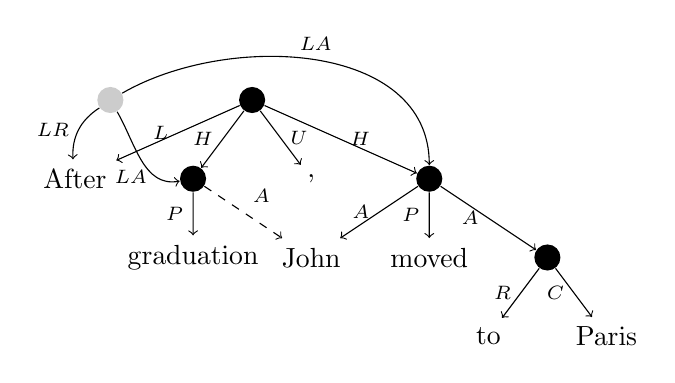
\begin{tikzpicture}[level distance=10mm, ->]
    \node (ROOT) [fill=black, circle] {}
      child {node (After) {After} edge from parent node[left] {\scriptsize $L$}}
      child {node (graduation) [fill=black, circle] {}
      {
        child {node {graduation} edge from parent node[left] {\scriptsize $P$}}
      } edge from parent node[left] {\scriptsize $H$} }
      child {node {,} edge from parent node[right] {\scriptsize $U$}}
      child {node (moved) [fill=black, circle] {}
      {
        child {node (John) {John} edge from parent node[left] {\scriptsize $A$}}
        child {node {moved} edge from parent node[left] {\scriptsize $P$}}
        child {node [fill=black, circle] {}
        {
          child {node {to} edge from parent node[left] {\scriptsize $R$}}
          child {node {Paris} edge from parent node[left] {\scriptsize $C$}}
        } edge from parent node[left] {\scriptsize $A$} }
      } edge from parent node[right] {\scriptsize $H$} }
      ;
    \draw[dashed,->] (graduation) to node [auto] {\scriptsize $A$} (John);
    \node (LKG) at (-1.8,0) [fill=black!20, circle] {};
    \draw[bend right] (LKG) to node [auto, left] {\scriptsize $LR$} (After);
    \draw (LKG) to[out=-60, in=190] node [below] {\scriptsize $LA\quad$} (graduation);
    \draw (LKG) to[out=30, in=90] node [above] {\scriptsize $LA$} (moved);
  \end{tikzpicture}
  }\caption{UCCA \label{fig:original_example_ucca}}
\end{subfigure}}

\fbox{\begin{subfigure}{0.47\textwidth}
  \centering
  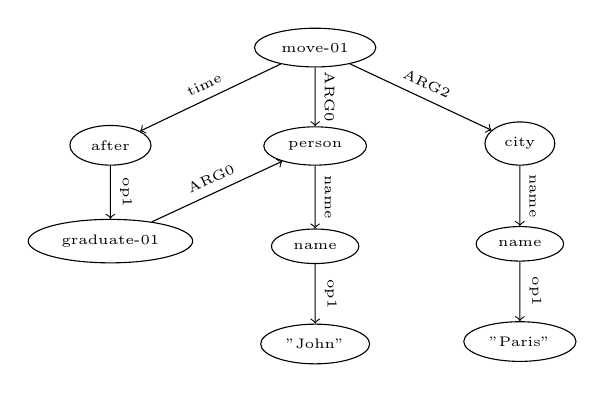
\begin{tikzpicture}[level distance=15mm, ->,
      every node/.append style={sloped,anchor=south,auto=false,font=\tiny},
      level 1/.style={sibling distance=26mm}]
    \node (ROOT) [draw=black,ellipse] {move-01}
      child {node [draw=black,ellipse] {after}
      {
            child {node (graduation) [draw=black,ellipse] {graduate-01} edge from parent node {op1} }
      } edge from parent node {time} }
      child {node (John) [draw=black,ellipse] {person}
      {
        child {node [draw=black,ellipse] {name}
        {
            child {node [draw=black,ellipse] {"John"} edge from parent node {op1} }
        } edge from parent node {name} }
      } edge from parent node {ARG0} }
      child {node [draw=black,ellipse] {city}
      {
        child {node [draw=black,ellipse] {name}
        {
            child {node [draw=black,ellipse] {"Paris"} edge from parent node {op1} }
        } edge from parent node {name} }
      } edge from parent node {ARG2} }
      ;
      \draw (graduation) to node {ARG0} (John);
  \end{tikzpicture}
  \caption{AMR \label{fig:original_example_amr}}
\end{subfigure}}

\fbox{\begin{subfigure}{0.47\textwidth}
  \centering
    \begin{dependency}[text only label, label style={above}, font=\small]
    \begin{deptext}[column sep=.8em,ampersand replacement=\^]
    After \^ graduation \^ , \^ John \^ moved \^ to \^ Paris \\
    \end{deptext}
        \depedge{1}{2}{ARG2}
        \depedge{5}{4}{ARG1}
        \depedge[edge unit distance=2ex]{1}{5}{ARG1}
        \deproot{5}{top}
        \depedge[edge unit distance=4ex, edge start x offset=-1ex]{5}{7}{ARG2}
        \depedge[edge start x offset=1ex]{6}{5}{ARG1}
        \depedge{6}{7}{ARG2}
    \end{dependency}
  \caption{DM \label{fig:original_example_sdp}}
\end{subfigure}}

\fbox{\begin{subfigure}{0.47\textwidth}
  \centering
    \begin{dependency}[text only label, label style={above}, font=\small]
    \begin{deptext}[column sep=.8em,ampersand replacement=\^]
    After \^ graduation \^ , \^ John \^ moved \^ to \^ Paris \\
    \end{deptext}
        \depedge{2}{1}{case}
        \depedge{4}{3}{punct}
        \depedge{5}{4}{nsubj}
        \depedge{2}{5}{obl}
        \depedge{7}{6}{case}
        \deproot{5}{root}
        \depedge{5}{7}{obl}
    \end{dependency}
  \caption{UD \label{fig:original_example_ud}}
\end{subfigure}}


\caption{\label{fig:original_examples}
 Example graph for each representation scheme we use.
 Figure \ref{fig:original_example_ucca} presents a UCCA graph. The dashed edge is remote,
  while the gray node and its outgoing edges represent inter-Scene linkage.
  Pre-terminal nodes and edges are omitted for brevity. 
 Figure \ref{fig:original_example_amr} presents an AMR graph.
  The text tokens are not part of the graph, and must be matched to
  concepts and constants by alignment. Variables are represented by their concepts.
 Figure \ref{fig:original_example_sdp} presents an SDP graph (in the DM formalism).
  The graph contains multiple roots: ``After'', ``moved'' and ``to''.
  One of the roots is marked as \textit{top}: ``moved''.
  Punctuation is not included in the graph as it is non-content-bearing.
 Figure \ref{fig:original_example_ud} presents a UD tree.
  Each word has exactly one head, and there is a single root.
  Edge labels correspond to syntactic relations.
}

\end{figure}


%%%%%%%%%%%%%%%%%%%%%%%%%%%%%%%%%%%%%%%%%%%%%%%%%%%%%%%%%%%%%%%%%%%%%%%%%%%%%%%%%
\section{Tackled Tasks}\label{sec:tasks}

In this section, we outline the parsing tasks we are addressing.
We focus on representation schemes that provide a full-sentence analysis,
i.e., schemes that produce a graph covering all (content) words in the text, 
or the lexical concepts they evoke.
Full-sentence analysis contrasts with ``shallow'' semantic parsing,
primarily Semantic Role Labeling
\cite[SRL;][]{Palmer:05,gildea2002automatic,swayamdipta2017frame,ringgaard2017sling},
which specifically targets argument structure phenomena using flat structures.
We consider four target representations: UCCA, DM, UD
\cite[Universal Dependencies; ][]{nivre2016universal}, and AMR.
Figure~\ref{fig:original_examples} presents the representations of the same sentence 
using each of the schemes.
%annotating the sentence ``After graduation, John moved to Paris''.

%Although each of these tasks uses different graph structures,
%they all involve whole-sentence (or whole-paragraph) semantic analysis,
%and due to the structure of phenomena such as predicate-argument relations,
%require parsers that can handle non-projectivity (or discontinuity) and reentrancy, resulting in
%directed acyclic graphs (DAGs).\oa{maybe add a diagram or at least elaborate more on these like we
%did in the TUPA paper, with examples etc.}

\paragraph{Universal Conceptual Cognitive Annotation.}\label{sec:ucca}
UCCA \cite{abend2013universal} is a semantic representation scheme whose main design principles
are ease of annotation, cross-linguistic applicability and stability, and a modular architecture of semantic distinctions.
UCCA represents the semantics of natural language utterances
as directed acyclic graphs (DAGs), where terminal nodes (nodes without children)
correspond to the text tokens, and non-terminal nodes to semantic units that participate
in some super-ordinate relation.
Edges are labeled, indicating the role of a child in the relation the parent represents.
Nodes and edges may belong to one of several \textit{layers}, each corresponding
to a ``module'' of semantic distinctions.
UCCA's \textit{foundational layer} (the only layer for which annotated data exists) 
mostly covers predicate-argument structure, semantic heads and inter-Scene relations.
%The \textit{linkage} layer covers relations between events, including temporal and discourse relations
%(exemplified by the gray node and its outgoing edges in Figure~\ref{fig:original_example_ucca}).

UCCA distinguishes \textit{primary} edges, corresponding 
to explicit relations, from \textit{remote} edges (appears dashed in
Figure~\ref{fig:original_example_ucca}) that allow for a unit to participate
in several super-ordinate relations.
Primary edges form a tree, whereas remote edges enable reentrancy, forming a DAG.
%As UCCA annotated data is currently fairly scarce (see \S\ref{sec:experiments}), 
%we hypothesize it will benefit from MTL, and consider it as our
%main task.

%%%%%%%%%%%%%%%%%%%%%%%%%%%%%%%%%%%%%%%%%%%%%%%%%%%%%%%%%%%%%%%%%%%%%%%%%%%%%5
\paragraph{Abstract Meaning Representation.}\label{sec:amr}

AMR \cite{banarescu2013abstract} is a semantic representation that encodes information about named entities, 
argument structure, semantic roles, word sense disambiguation and co-reference resolution.
AMRs are rooted directed graphs, in which both nodes and edges are labeled.
Most AMRs are DAGs, although cycles are permitted.

AMR differs from the other schemes we consider in that it does not anchor its graphs
in the words of the sentence (Figure~\ref{fig:original_example_amr}). Instead, AMR graphs
connect variables, concepts (from a pre-defined set) and constants (which may be strings or numbers).
Still, most AMR nodes are alignable to text tokens, a tendency used by AMR parsers,
that align a sub-set of the graph nodes to a sub-set of the text tokens (concept identification). In this work, we use pre-aligned AMR graphs.

Despite the brief period since its inception, AMR has been targeted by a number of works,
notably in two SemEval shared tasks \cite{may2016semeval,may2017semeval}.
In order to tackle the variety of distinctions it encodes and the unrestricted graph structure
it uses, AMR parsers often use specialized methods.
Graph-based parsers construct AMRs
by identifying concepts and scoring edges between them, either in a pipeline fashion
\cite{flanigan2014discriminative,artzi2015broad,pust2015parsing,foland2017abstract},
or jointly \cite{zhou2016amr}.
Another line of work %uses sequence-to-sequence models \cite{sutskever2014sequence},
trains machine translation models to convert strings into linearized AMRs
%treating AMR parsing as a machine translation model and linearizing the graph structure
\cite{barzdins2016riga,Gildea2017AddressingTD,Konstas2017NeuralAS,Buys2017RobustIN}.
Transition-based AMR parsers either 
use dependency trees as pre-processing, then mapping them into AMRs
\cite{wang-xue-pradhan:2015:ACL-IJCNLP,wang2015transition,wang-EtAl:2016:SemEval,goodman2016noise},
or use a transition system tailored to AMR parsing \cite{damonte-17,D17-1130}.
We differ from the above approaches in addressing AMR parsing 
using the same general DAG parser used for other schemes.


%%%%%%%%%%%%%%%%%%%%%%%%%%%%%%%%%%%%%%%%%%%%%%%%%%%%%%%%%%%%%%%%%%%%%%%%%%%%%5
\paragraph{Semantic Dependency Parsing.}\label{sec:sdp}

SDP uses a set of related representations, targeted in two recent SemEval shared tasks 
\cite{oepen2014semeval,oepen2015semeval}, and extended by \citet{oepen2016towards}.
They correspond to four semantic representation schemes, referred to as
DM, PAS, PSD and CCD, representing
predicate-argument relations between content-bearing words in a sentence.
All are based on semantic formalisms whose annotation has been
converted into bilexical dependencies---labeled
directed graphs whose nodes are all text tokens.
Edges are labeled, encoding semantic relations between the tokens.
Non-content tokens, such as punctuation,
are often left out of the analysis (see Figure~\ref{fig:original_example_sdp}),
but the sub-graph restricted to content-bearing tokens is connected.
Graphs containing cycles have been removed from the SDP datasets.

We consider one of the four formalisms used
in the SemEval shared tasks: DM (DELPH-IN MRS) representation, which was converted from 
DeepBank \cite{flickinger2012deepbank}, a corpus of hand-corrected parses from the LinGO
English Resource Grammar \cite{copestake2000open}.
LinGO is an HPSG grammar \cite{pollard1994head}
which uses Minimal Recursion Semantics \cite{copestake2005minimal}.


%%%%%%%%%%%%%%%%%%%%%%%%%%%%%%%%%%%%%%%%%%%%%%%%%%%%%%%%%%%%%%%%
\paragraph{Universal Dependencies.}\label{sec:ud}
UD \cite{nivre2016universal,11234/1-2515} has quickly become
the dominant dependency representation for
syntactic treebank annotation in a large variety of languages,
aiming for cross-linguistically consistent and coarse-grained treebank
annotation. Formally, UD uses bilexical trees, with edge labels 
representing syntactic relations between words.

While not a semantic representation,
we use UD as an auxiliary task,
inspired by previous work on joint syntactic and semantic parsing
(see \S\ref{sec:related_work}).
%\cite{lluis2008joint,collobert2011natural,D15-1169,swayamdipta-EtAl:2016:CoNLL,swayamdipta2017frame}.
In order to reach comparable analyses cross-linguistically,
UD often ends up in annotation that is similar to the common practice
in semantic treebanks, such as linking content words to content words wherever possible.
Using UD further allows conducting experiments on French and German, 
for which SDP and AMR annotated data is not available (\S\ref{sec:results}).

In addition to basic UD trees, we use the \textit{enhanced++} UD graphs available for English,
which are generated by the Stanford CoreNLP converters \cite{SCHUSTER16.779}.
These include additional and augmented relations between content words,
partially overlapping with the notion of remote edges in UCCA:
in the case of control verbs, for example, a direct relation is added in 
enhanced UD between the subordinated verb and its controller,
which is similar to the semantic schemes' treatment of this construction.


%%%%%%%%%%%%%%%%%%%%%%%%%%%%%%%%%%%%%%%%%%%%%%%%%%%%%%%%%%%%%%%%%%%%%%%%%%%%%%%%%%%%%%%%
\section{General Transition-based DAG Parser}\label{sec:model}

All schemes we outlined in \S\ref{sec:tasks} exhibit
reentrancy and discontinuity (or non-projectivity), to varying degrees.
In addition, UCCA and AMR contain non-terminal nodes.
In order to parse graphs with these structural properties,
we extend TUPA \cite[henceforth HAR17]{hershcovich2017a}, 
a transition-based parser 
originally developed for UCCA,
as it is the only parser to our knowledge that supports 
all these structural properties.
TUPA's transition system can yield any labeled DAG structure
whose leaves are aligned to text tokens.
To support parsing into AMR, which uses graphs that are not anchored in the tokens,
 we take advantage of existing alignments of the graphs with the text
tokens during training (\S\ref{sec:format}).

First used for projective syntactic dependency tree parsing \cite{Nivre03anefficient},
transition-based parsers have since been generalized to parse into many other
graph families, such as (discontinuous) constituency trees \cite[e.g., ][]{zhang2009transition,maier-lichte:2016:DiscoNLP},
and DAGs \cite[e.g.,][]{sagae2008shift,du-EtAl:2015:SemEval}. %ribeyre-villemontedelaclergerie-seddah:2014:SemEval,

Transition-based parsers apply \textit{transitions}
incrementally to an internal state defined by a buffer $B$ of remaining tokens 
and nodes, a stack $S$ of incomplete nodes, and a labeled graph $G$ of 
constructed nodes and edges.
When a terminal state is reached, the graph $G$ is the final output.
A classifier is used at each step to select the next transition, 
based on features that encode the current state.
%During training, an oracle converts the gold-standard annotations into
% training instances.




\subsection{TUPA's Transition Set}\label{sec:transition_set}

Given a sequence of tokens $w_1, \ldots, w_n$,
we predict a rooted graph $G$ whose terminals are the tokens.
Parsing starts with the root node on the stack,
and the input tokens in the buffer.

The TUPA transition set includes
the standard \textsc{Shift} and \textsc{Reduce} operations,
\textsc{Node$_X$} for creating a new non-terminal node and an $X$-labeled edge,
\textsc{Left-Edge$_X$} and \textsc{Right-Edge$_X$} to create a new primary $X$-labeled edge,
\textsc{Left-Remote$_X$} and \textsc{Right-Remote$_X$} to create a new remote $X$-labeled edge,
\textsc{Swap} to handle discontinuous nodes,
and \textsc{Finish} to mark the state as terminal.

Although UCCA contains nodes without any text tokens as descendants
(called \textit{implicit units}),
these nodes are infrequent and only cover 0.5\% of the non-terminal nodes.
For this reason we follow HAR17 and discard implicit units from the training and evaluation,
and so do not include transitions for creating them.
% when parsing UCCA,
%thus ignoring them in both training and evaluation.
%We also adopt the standard evaluation for UCCA parsing, which is span-based,
%and ignores implicit units as well. 

In AMR, implicit units are considerably more common, as any unaligned concept
with no aligned descendents is implicit (about 6\% of the nodes).
Implicit AMR nodes usually result from alignment errors, or from abstract concepts
which have no explicit realization in the text \cite{buys2017oxford}.
We ignore implicit nodes when training on AMR as well.
TUPA also does not support node labels, 
which are ubiquitous in AMR but absent in UCCA structures (only edges are labeled in UCCA). 
We therefore only produce edge labels and not node labels when training on AMR.

\begin{figure}[t]
   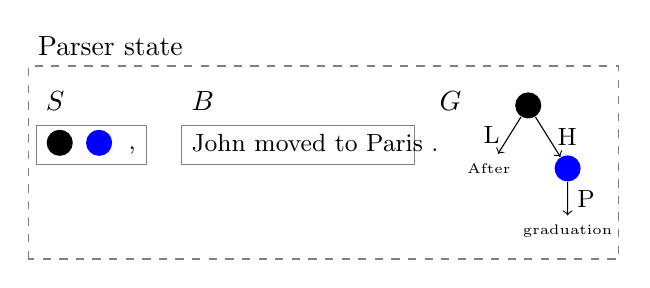
\begin{tikzpicture}[level distance=8mm, sibling distance=1cm]
   \node[anchor=west] at (0,1.5) {Parser state};
   \draw[color=gray,dashed] (0,-1.2) rectangle (7.5,1.25);
   \draw[color=gray] (.1,0) rectangle (1.5,.5);
   \node[anchor=west] at (.1,.8) {$S$};
   \node[fill=black, circle] at (.4,.275) {};
   \node[fill=blue, circle] at (.9,.275) {};
   \node[anchor=west] at (1.15,.175) {\small ,};
   \draw[color=gray] (1.95,0) rectangle (4.9,.5);
   \node[anchor=west] at (1.95,.8) {$B$};
   \node[anchor=west] at (1.95,.275) {\small John moved to Paris .};
   \node[anchor=west] at (5.1,.8) {$G$};
   \node[fill=black, circle] at (6.35,.75) {}
     child {node  {\tiny After} edge from parent [->] node[left] {\small L}}
     child {node [fill=blue, circle] {}
     {
       child {node {\tiny graduation} edge from parent [->] node[right] {\small P}}
     } edge from parent [->] node[right] {\small H} };
   \end{tikzpicture}
   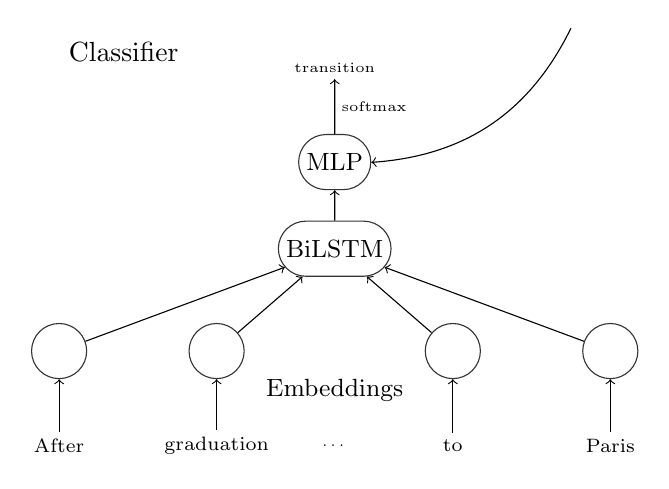
\begin{tikzpicture}[->]
   \node[anchor=west] at (0,6) {Classifier};
   \tiny
   \tikzstyle{main}=[rounded rectangle, minimum size=7mm, draw=black!80, node distance=12mm]
   \node[main] (specific) at (3.5,3.5) {\small BiLSTM};
   \node (embeddings) at (3.5,1.7) {\small Embeddings};
   \foreach \i/\word in {0/{After},2/{graduation},5/{to},7/{Paris}} {
       \node (x\i) at (\i,1) {\scriptsize \word};
       \node[main] (e\i) at (\i,2.2) {};
       \path (x\i) edge (e\i);
       \path (e\i) edge (specific);
   }
    \node (x4) at (3.5,1) {\ldots};
    \node[main] (mlp) at (3.5,4.6) {\small MLP};
    \path (specific) edge (mlp);
    \coordinate (state) at (6.5,6.3);
    \path (state) edge [bend left] (mlp);
    \node (transition) at (3.5,5.8) {transition};
    \path (mlp) edge node[right] {softmax} (transition);
   \end{tikzpicture}
\caption{Illustration of the TUPA model, adapted (with permission) from \citet{hershcovich2017a}.
Top: parser state.
Bottom: BiLTSM architecture.}
\label{fig:single_model}
\end{figure}


%%%%%%%%%%%%%%%%%%%%%%%%%%%%%%%%%%%%%%%%%%%%%%%%%%%%%%%%%%%%%%%%%%%%%%%%%%%%%%%%%
\subsection{Transition Classifier}\label{sec:classifier}

To predict the next transition at each step,
we use a BiLSTM with embeddings as inputs,
followed by an MLP and a softmax layer for classification 
(see Figure~\ref{fig:single_model}).
Inference is performed greedily,
and training is done with an oracle that yields the set of all optimal 
transitions at a given state (those from which the gold graph is still reachable).
Out of this set, the actual transition performed in training is the one
with the highest score given by the classifier,
which is trained to maximize the sum of log-likelihoods of all 
optimal transitions at each step.


\begin{figure}
\fbox{\begin{subfigure}{0.47\textwidth}
    \centering
    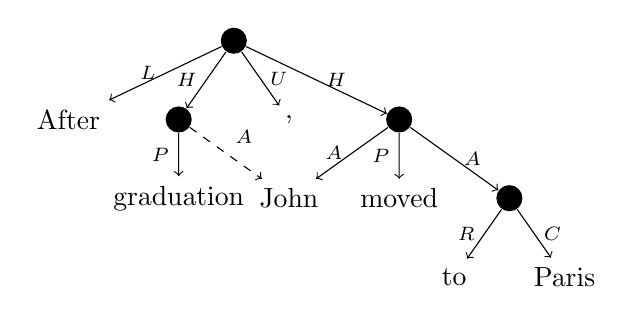
\begin{tikzpicture}[level distance=10mm, sibling distance=14mm, ->,
        every circle node/.append style={fill=black}]
      \tikzstyle{word} = [font=\rmfamily,color=black]
      \node (ROOT) [circle] {}
        child {node (After) [word] {After} edge from parent node[left] {\scriptsize $L$}}
        child {node (graduation) [circle] {}
        {
          child {node [word] {graduation} edge from parent node[left] {\scriptsize $P$}}
        } edge from parent node[left] {\scriptsize $H$} }
        child {node [word] {,} edge from parent node[right] {\scriptsize $U$}}
        child {node (moved) [circle] {}
        {
          child {node (John) [word] {John} edge from parent node[left] {\scriptsize $A$}}
          child {node [word] {moved} edge from parent node[left] {\scriptsize $P$}}
          child {node [circle] {}
          {
            child {node [word] {to} edge from parent node[left] {\scriptsize $R$}}
            child {node [word] {Paris} edge from parent node[right] {\scriptsize $C$}}
          } edge from parent node[right] {\scriptsize $A$} }
        } edge from parent node[right] {\scriptsize $H$} }
        ;
      \draw[dashed,->] (graduation) to node [auto] {\scriptsize $A$} (John);
    \end{tikzpicture}
  \caption{UCCA}
  \label{fig:converted_example_ucca}
\end{subfigure}}

\fbox{\begin{subfigure}{0.47\textwidth}
  \centering
  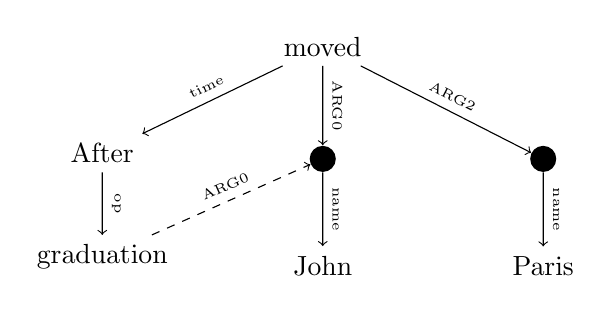
\begin{tikzpicture}[level distance=16mm, ->,
      every node/.append style={sloped,anchor=south,auto=false,font=\tiny},
      level 1/.style={sibling distance=28mm},
      level 2/.style={sibling distance=14mm},
      level 3/.style={sibling distance=12mm}]
    \tikzstyle{word} = [font=\rmfamily,color=black]
    \node (ROOT) [word] {moved}
      child {node [word] {After}
      {
            child {node (graduation) [word] {graduation} edge from parent node {op} }
      } edge from parent node {time} }
      child {node (John) [fill=black,circle] {}
      {
        child {node [word] {John} edge from parent node {name} }
      } edge from parent node {ARG0} }
      child {node [fill=black,circle] {}
      {
        child {node [word] {Paris} edge from parent node {name} }
      } edge from parent node {ARG2} }
      ;
      \draw[dashed] (graduation) to node {ARG0} (John);
  \end{tikzpicture}
  \captionof{figure}{AMR}
  \label{fig:converted_example_amr}
\end{subfigure}}

\fbox{\begin{subfigure}{0.47\textwidth}
  \centering
  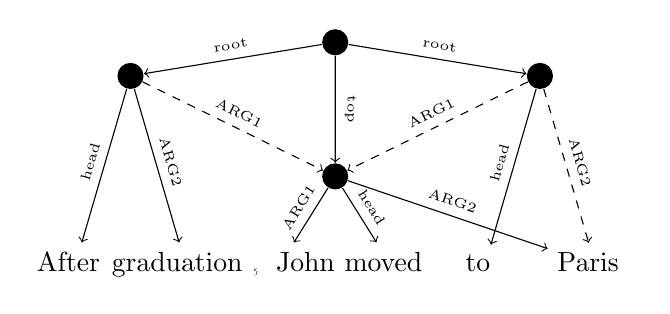
\begin{tikzpicture}[level distance=12mm, ->,
      every node/.append style={sloped,anchor=south,auto=false,font=\tiny},
      level 1/.style={sibling distance=26mm,level distance=6mm},
      level 2/.style={sibling distance=14mm,level distance=14mm}]
    \tikzstyle{word} = [font=\rmfamily,color=black]
    \node (ROOT) [fill=black,circle] {}
      child {node (after) [fill=black,circle] {}
      {
        child {node [draw=none] {}
        {
          child {node [word] (after_word) {After{\color{white}g}} edge from parent [draw=none]}
        } edge from parent [draw=none] }
        child {node [draw=none] {}
        {
          child {node [word] (graduation) {graduation ,} edge from parent [draw=none]}
        } edge from parent [draw=none] }
      } edge from parent node {root}}
      child {node [draw=none] {}
      {
        child {node (moved) [fill=black,circle] {}
        {
          child {node [word] {\quad{\color{white}g} John} edge from parent node {ARG1}}
          child {node [word] {moved{\color{white}g}} edge from parent node {head}}
        } edge from parent [draw=none] }
      } edge from parent [draw=none] }
      child {node (to) [fill=black,circle] {}
      {
        child {node [draw=none] {}
        {
            child {node [word] (to_word) {to{\color{white}g}} edge from parent [draw=none]}
          } edge from parent [draw=none] }
          child {node [draw=none] {}
        {
          child {node [word] (Paris) {Paris{\color{white}g}} edge from parent [draw=none]}
        } edge from parent [draw=none] }
      } edge from parent node {root}}
      ;
      \draw (ROOT) to node {top} (moved);
      \draw (after) to node {head} (after_word);
      \draw (after) to node {ARG2} (graduation);
      \draw[dashed] (after) to node {ARG1} (moved);
      \draw[dashed] (to) to node {ARG1} (moved);
      \draw (to) to node {head} (to_word);
      \draw (moved) to node {ARG2} (Paris);
      \draw[dashed] (to) to node {ARG2} (Paris);
  \end{tikzpicture}
  \captionof{figure}{DM}
  \label{fig:converted_example_sdp}
\end{subfigure}}

\fbox{\begin{subfigure}{0.47\textwidth}
  \centering
  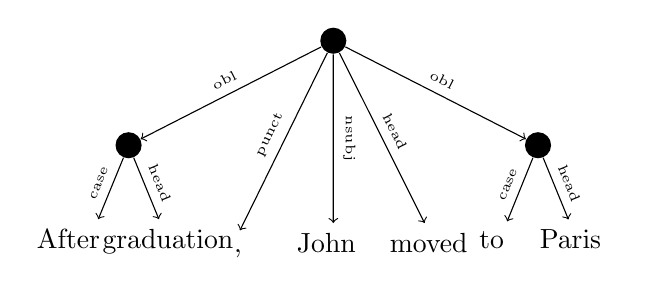
\begin{tikzpicture}[level distance=15mm, ->,
      every node/.append style={sloped,anchor=south,auto=false,font=\tiny},
      level 1/.style={sibling distance=13mm},
      level 2/.style={sibling distance=1cm}]
    \tikzstyle{word} = [font=\rmfamily,color=black]
    \node (ROOT) [fill=black,circle] {}
      child {node (after) [fill=black,circle] {}
      {
        child {node [word] {After{\color{white}g}\quad\quad} edge from parent node {case}}
        child {node [word] {\quad graduation\quad\quad} edge from parent node {head}}
      } edge from parent node {obl}}
      child {node {}
      {
        child {node [word] (comma) {\quad,{\color{white}g}} edge from parent [draw=none]}
      } edge from parent [draw=none]}
      child {node {}
      {
        child {node [word] (John) {John{\color{white}g}} edge from parent [draw=none]}
      } edge from parent [draw=none]}
      child {node {}
      {
        child {node [word] (moved) {moved{\color{white}g}} edge from parent [draw=none]}
      } edge from parent [draw=none]}
      child {node (to) [fill=black,circle] {}
      {
          child {node [word] {to{\color{white}g}} edge from parent node {case}}
          child {node [word] {Paris{\color{white}g}} edge from parent node {head}}
      } edge from parent node {obl}}
      ;
      \draw (ROOT) to node {punct} (comma);
      \draw (ROOT) to node {nsubj} (John);
      \draw (ROOT) to node {head} (moved);
  \end{tikzpicture}
  \captionof{figure}{UD}
  \label{fig:converted_example_ud}
\end{subfigure}}

\caption{Graphs from Figure~\ref{fig:original_examples}, after conversion to the the unified DAG format
(pre-terminals omitted: each terminal drawn in place of its parent).
Figure~\ref{fig:converted_example_ucca} presents a converted UCCA graph.
Linkage nodes and edges are removed, but the original graph is otherwise preserved.
Figure~\ref{fig:converted_example_amr} presents a converted AMR graph, with
text tokens added according to the alignments.
Numeric suffixes of \textit{op} relations were removed,
and names collapsed.
Figure~\ref{fig:converted_example_sdp} presents a converted SDP graph (in the DM formalism), with
intermediate non-terminal nodes introduced as \textit{head} units.
In case of reentrancy, an arbitrary reentrant edge is marked as remote.
Figure~\ref{fig:converted_example_ud} presents a converted UD graph.
As in SDP, intermediate non-terminals and \textit{head} edges are introduced.
The graph is actually a tree, as was the original bilexical graph.
}
\label{fig:converted_examples}
\end{figure}


\paragraph{Features.}
We use features from HAR17,
representing the words, POS tags, syntactic dependency relations, and previously predicted edge labels
for nodes in specific locations in the parser state.
In addition, for each token
we use embeddings representing the one-character prefix, three-character suffix,
shape (capturing orthographic features, e.g. "Xxxx" or "dd"),
and named entity type,\footnote{See Supplementary Material for a full listing of features.}
all provided by spaCy \cite{spacy2}.\footnote{\url{http://spacy.io}}
To the learned word vectors, we also concatenate the 250K most frequent word vectors from fastText
\cite{bojanowski2016enriching},\footnote{\url{http://fasttext.cc}}
pre-trained over Wikipedia and updated during training.
%For AMR we add node label features according to gold node labels.


\paragraph{Constraints.}
As each annotation scheme has different constraints on the allowed graph structures,
we define these constraints separately for each task.
During training and parsing, the relevant constraint set rules out some of the transitions
according to the parser state.


Some constraints are task-specific, others are generic.
For example, in UCCA, a terminal may only have one parent.
In AMR, a concept corresponding to a PropBank frame may only have 
the core arguments defined for the frame.
An example generic constraint is that stack nodes 
that have been swapped
should not be swapped again.\footnote{
 To implement this constraint, we define a \textit{swap index}
 for each node, assigned when the node is created.
 At initialization, only the root node and terminals exist.
 We assign the root a swap index of 0, and for each terminal, its
 position in the text (starting at 1).
 Whenever a node is created as a result of a \textsc{Node}
 transition, its swap index is the arithmetic
 mean of the swap indices of the stack top and buffer head.}


%%%%%%%%%%%%%%%%%%%%%%%%%%%%%%%%%%%%%%%%%%%%%%%%%%%%%%%%%%%%%%%%%%%%%%%%%%%%%%%%%%%%%%%%
\section{Unified DAG Format}\label{sec:format}

To be able to use TUPA for the four tasks presented in \S\ref{sec:tasks},
we convert them all into a unified DAG format, which is inclusive enough to
allow representing any of the schemes with very little loss of information.\footnote{See
Supplementary Material for conversion details.}

The format consists of a rooted DAG, where the tokens are the terminal nodes.
As in the UCCA format, the edges (but not the nodes) are labeled,
and are divided into \textit{primary} and \textit{remote} edges,
where the primary edges form a tree (all nodes have at most one primary parent,
and the root has none).
The remote edges enable reentrancy, and thus together with primary edges
form a DAG.
Figure~\ref{fig:converted_examples} shows examples for converted graphs.
Converting UCCA into the unified format consists simply of removing linkage 
nodes and edges (see Figure~\ref{fig:converted_example_ucca}), which were
also discarded by HAR17.

\paragraph{Converting bilexical dependencies.}
In order to convert DM and UD into the unified DAG format,
we add a pre-terminal for each token,
and then attach the pre-terminals according to the original dependency edges:
traversing the tree from the root down, for each head token we create a non-terminal
parent with the edge label {\it head},
and add the node's dependents as children of the created non-terminal node
(see Figures~\ref{fig:converted_example_sdp} and \ref{fig:converted_example_ud}).
Since DM allows multiple roots, we form a single root node, whose children
are the original roots. The added edges are labeled \textit{root}, where
top nodes are labeled \textit{top} instead.
In case of reentrancy, an arbitrary parent is marked as primary, and the rest as remote
(denoted as dashed edges in Figure~\ref{fig:converted_examples}).

\paragraph{Converting AMR.}
In the conversion from AMR, non-terminals are already present, and node labels are dropped.
However, alignments must be handled (see Figure~\ref{fig:converted_example_amr}).
Since alignment between nodes and text tokens is not part of the AMR graph,
we insert the alignments into the graph as edges in the conversion.
Specifically, we use automatically pre-aligned graphs (see \S\ref{sec:experiments}),
and attach each node with an edge labeled \textit{Terminal} to each of the terminals it is aligned to.
%
%Since the order of AMR ordinal relations, such as \textit{op1}, \textit{op2},
%is annotated according to the order of text tokens,
%the numeric index is redundant and is thus removed.
%Numeric suffixes are kept when they are meaningful, e.g. in distinguishing between PropBank semantic
%roles (\textit{ARG[0-5]}).
Named entities in AMR are represented as a sub-graph, whose \textit{name}-labeled root
has a child for each token in the name (see the two \textit{name} nodes in Figure~\ref{fig:original_example_amr}).
We collapse this sub-graph into a single node whose children are the name tokens.


\begin{figure}[t]
   \begin{tikzpicture}
   \node[anchor=west] at (0,1) {Parser state};
   \draw[color=gray,dashed] (0,0) rectangle (7.5,.75);
    \node (x4) at (3.75,0.375) {\ldots};
   \end{tikzpicture}
   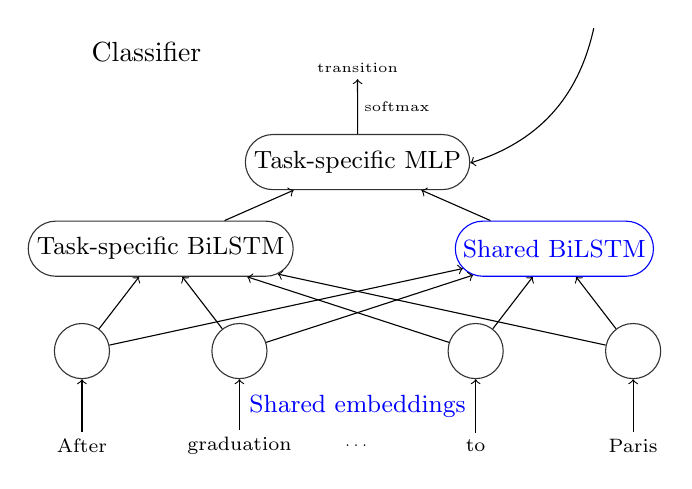
\begin{tikzpicture}[->]
   \node[anchor=west] at (0,6) {Classifier};
   \tiny
   \tikzstyle{main}=[rounded rectangle, minimum size=7mm, draw=black!80, node distance=12mm]
   \node[main] (specific) at (1,3.5) {\small Task-specific BiLSTM};
   \node[main,color=blue] (shared) at (6,3.5) {\small Shared BiLSTM};
   \node[color=blue] (embeddings) at (3.5,1.5) {\small Shared embeddings};
   \foreach \i/\word in {0/{After},2/{graduation},5/{to},7/{Paris}} {
       \node (x\i) at (\i,1) {\scriptsize \word};
       \node[main] (e\i) at (\i,2.2) {};
       \path (x\i) edge (e\i);
       \path (e\i) edge (specific);
       \path (e\i) edge (shared);
   }
    \node (x4) at (3.5,1) {\ldots};
    \node[main] (mlp) at (3.5,4.6) {\small Task-specific MLP};
    \path (specific) edge (mlp);
    \path (shared) edge (mlp);
    \coordinate (state) at (6.5,6.3);
    \path (state) edge [bend left] (mlp);
    \node (transition) at (3.5,5.8) {transition};
    \path (mlp) edge node[right] {softmax} (transition);
   \end{tikzpicture}
   \caption{MTL model.
      Input token representations are computed both by a task-specific and a shared BiLSTM.
      Their outputs are concatenated with the embedding of the parser state and fed into the task-specific MLP for selecting the next transition.}
   \label{fig:multi_model}
\end{figure}


%%%%%%%%%%%%%%%%%%%%%%%%%%%%%%%%%%%%%%%%%%%%%%%%%%%%%%%%%%%%%%%%%%%%%%%%%%%%%%%%%%%%%%%%%%%%
\section{Multitask Transition-based Parsing}\label{sec:multitask}

Since the same TUPA model can be applied to different tasks, 
we can train it in a multitask setting.
Following previous work, we share only some of the model parameters
\cite{N16-1179,P16-2038,C16-1013,C16-1059,C16-1179,E17-1005,P17-1186}, leaving task-specific
sub-networks as well.
Concretely, we replicate the BiLSTM used by TUPA for each of the tasks, and additionally add
a BiLSTM which is shared across all tasks. 
For each task, the outputs of the task-specific and shared BiLSTMs are concatenated and
fed into a task-specific MLP (see Figure~\ref{fig:multi_model}).
Feature embeddings are shared across tasks.

The fairly small training set available for UCCA (see \S\ref{sec:experiments})
makes MTL particularly appealing,
and we focus on it in this paper, treating AMR, DM and UD parsing as auxiliary tasks.

\paragraph{Unlabeled parsing for auxiliary tasks.}
In order to simplify the auxiliary tasks and facilitate generalization \cite{E17-2026,E17-1005},
we perform unlabeled parsing for AMR, DM and UD in the multitask setting,
while still predicting edge labels in UCCA parsing.
To support unlabeled parsing, we simply remove all labels from the
\textsc{Edge}, \textsc{Remote} and \textsc{Node} transitions outputted by the oracle.
This results in a much smaller number of transitions the classifier has to select from
(no more than 10, as opposed to 45 transitions in labeled UCCA parsing),
allowing us to use fewer dimensions and layers for the task-specific BiLSTMs and MLPs
of the auxiliary tasks (see Supplementary Material).
This limited capacity forces the network to use the shared parameters for all tasks,
increasing generalization \cite{E17-1005}.



\section{Experiments}\label{sec:experiments}

We perform various experiments to assess the value of MTL to UCCA parsing,
training the parser in a single-task and multitask setting
and evaluating its performance on the UCCA test sets, in both in-domain and out-of-domain settings.

\begin{table}[t]
\centering
\small
\setlength\tabcolsep{3pt}
\begin{tabular}{l|rr|rr|rr}
& \multicolumn{2}{c|}{\footnotesize \bf English} & \multicolumn{2}{c|}{\footnotesize \bf French} & \multicolumn{2}{c}{\footnotesize \bf German} \\
\footnotesize \bf Corpus & \footnotesize \bf {\#}tok & \footnotesize \bf {\#}sent & \footnotesize \bf {\#}tok & \footnotesize \bf {\#}sent & \footnotesize \bf {\#}tok & \footnotesize \bf {\#}sent \\
\hline
\textbf{UCCA} &&&& \\
Wiki & 158433 & 5225 &&&& \\
20K & 12339 & 506 & 12929 & 547 & 153581 & 6935 \\
\hline
\textbf{UD} & 568560 & 24276 & 1114312 & 40102 & 318847 & 16590 \\
\hline
\textbf{AMR} & 708701 & 39260 \\
\hline
\textbf{DM} & 802717 & 35657 \\
\end{tabular}
\caption{Overall size of each corpus: total number of tokens ({\#}tok) and sentences ({\#}sent).
%\textit{Wiki} is the UCCA English Wikipedia corpus, and
%\textit{20K} is the UCCA English \textit{Twenty Thousand Leagues Under the Sea} corpus.
%We use UD v2.1, AMR release LDC2017T10 and SDP 2016 data for DM.
\label{tab:corpora}}
\end{table}

\paragraph{Data.}

For UCCA, we use the English Wikipedia corpus \cite[v1.0; ][]{abend2013universal},
with the standard train/dev/test split of 4254/453/518 sentences,
and the \textit{Twenty Thousand Leagues Under the Sea} corpus
\cite[\textit{20K Leagues};][]{sulem2015conceptual},
annotated in English, French and German.\footnote{\mbox{\url{http://github.com/huji-nlp/ucca-corpus}}}
The English part (v1.0) of \textit{20K Leagues} is used only as an out-of-domain test set, as in HAR17.
For the fairly small French part (v1.0; see Table~\ref{tab:corpora})
we use a train/dev/test split of 413/67/67 sentences.
For the German part (v0.9), which is noisy as it is still being developed,
we use a split of 4196/561/2174 sentences.
We tune on the respective development sets without cross-validation.

For AMR, we use LDC2017T10, identical to the dataset targeted in SemEval 2017
\cite{may2017semeval}.\footnote{\mbox{\url{http://catalog.ldc.upenn.edu/LDC2017T10}}}
For SDP, we use the DM target representation from the SDP 2016 dataset
\cite{oepen2016towards}.\footnote{\url{http://sdp.delph-in.net/osdp-12.tgz}}
For Universal Dependencies, we use all English, French and German treebanks from UD v2.1
\cite{11234/1-2515}.\footnote{\url{http://hdl.handle.net/11234/1-2515}}
We use the enhanced++ UD representation \cite{SCHUSTER16.779} in our English experiments,
henceforth referred to as UD$^{++}$.
For AMR, DM and UD, we use the training sets from standard train/dev/test splits.

While UCCA is annotated over Wikipedia and over a literary corpus,
the domains for AMR, DM and UD are blogs, news, emails, reviews, and Q\&A.
This domain difference between training and test is particularly challenging (see \S\ref{sec:discussion}).

\paragraph{Experimental setup.}

As our main experiment, we evaluate our method in settings where MTL tends to be the most effective:
in an out-of-domain setting (on English),
training on \textit{Wiki} and evaluating on \textit{20K Leagues};
and where the only available training data is very small (French)
or noisy (German), training on the \textit{20K Leagues} training sets and evaluating on the test sets.
We use unlabeled AMR, DM and UD$^{++}$ parsing as auxiliary tasks in English,
and unlabeled UD parsing in French and German.\footnote{We did not use AMR, DM or UD$^{++}$ in French
and German, as these are only available in English.}
Fur completeness, we also evaluate the English models on the \textit{Wiki} in-domain test set.


\paragraph{Evaluation.}

We evaluate on UCCA using labeled precision, recall and $F_1$ (harmonic mean of precision and recall)
on primary and remote edges,
following previous work on UCCA parsing \cite{hershcovich2017a}.
Edges in predicted and gold graphs are matched by terminal yield and label.



\paragraph{Training.}

Training proceeds by creating a unified corpus, shuffling all sentences from relevant
datasets together (according to the setting),
but using only the score on the UCCA development set as the criterion for early stopping.
In each training epoch, we use the same number of examples from each task---the
number of sentences in the UCCA training set.
Since training sets differ in size, we sample this many sentences from each training set.

All embeddings are initialized randomly.
We use dropout \cite{srivastava2014dropout} between MLP layers, and recurrent dropout
\cite{NIPS2016_6241} between BiLSTM layers, both with a probability of 0.4.
In addition, we use word, tag and dependency relation dropout \cite{kiperwasser2016simple}.\footnote{In
training, the embedding for a feature value $w$ is replaced with a zero vector
with a probability of $\frac{0.2}{\#(w)+0.2}$, where $\#(w)$ is the number of occurrences of
$w$ observed.}
For optimization we use a minibatch size of 100, decaying all weights by $10^{-5}$ at each update,
and train with stochastic gradient descent for 30 epochs with a learning
rate of 0.1, followed by AMSGrad \cite{j.2018on} for 30 epochs with
$\alpha=0.001,\beta_1=0.9$ and $\beta_2=0.999$.
We found this training strategy to work better than using only one of the optimization methods,
similar to findings by \citet{keskar2017improving}.
We select the epoch with the best average labeled $F_1$ score on the UCCA development set.
The neural network is implemented using DyNet \cite{neubig2017dynet}.\footnote{\url{http://dynet.io}}
See Supplementary Material for hyperparameter settings.

%\subsection{Ensembling}
%
%During inference, we use Product of Experts \cite[PoE; ][]{hinton2002training} to combine the predictions
%of three models trained in the same setting, but with different random seeds. The transition selected is
%\[
%\argmax_{t\in T}\sum_{i=1}^3\big[\log(\mathrm{softmax}(m_i(s)))\big]_t
%\]
%where $T$ is the set of possible transitions, $m_i$ are the combined models, and $s$ is the current state.
%
%In order to ensemble multitask models, we combine models trained with the same auxiliary task.
%Another alternative is to combine models trained with different auxiliary tasks.\oa{don't write about alternatives,
%but rather on what we actually do}
%This provides greater variability between the combined models.


\begin{table}[t]
\centering
\small
\setlength\tabcolsep{3pt}
\begin{tabular}{l|lll|lll}
& \multicolumn{3}{c|}{\footnotesize \bf Primary} & \multicolumn{3}{c}{\footnotesize \bf Remote} \\
& \footnotesize \textbf{LP} & \footnotesize \textbf{LR} & \footnotesize \textbf{LF}
& \footnotesize \textbf{LP} & \footnotesize \textbf{LR} & \footnotesize \textbf{LF} \\
\hline
\multicolumn{4}{l|}{\small \bf English (out-of-domain)} & \\
\footnotesize HAR17
& 68.7 & 68.5 & 68.6 & 38.6 & 18.8 & 25.3 \\
\footnotesize Single
& 68.9 & 68.9 & 68.9 & 40.7 & 19.6 & 26.5 \\
\cline{1-1}
%Single-task (PoE) & 69.7 & 69.5 & 69.6 & 50.5 & 19.4 & 28 \\
%\small \bf Multitask &&& \\
\footnotesize AMR
& 69.4 & 69.6 & 69.5 & 44.3 & 21.4 & 28.8 \\
\footnotesize DM
& 70.1$\star$ & 69.5 & 69.8$\star$ & 40 & 18.6 & 25.4 \\
\footnotesize UD$^{++}$
& 69.8$\star$ & 69.9$\star$ & 69.9$\star$ & 39.1 & 14.3$\dagger$ & 20.9$\dagger$ \\
\footnotesize AMR + DM
& 70.8$\star$ & 70$\star$ & 70.4$\star$ & 49.5$\star$ & 21 & 29.5 \\
\footnotesize AMR + UD$^{++}$
& 69.7$\star$ & 70$\star$ & 69.8$\star$ & 39 & 21.4 & 27.6 \\
\footnotesize DM + UD$^{++}$
& 70$\star$ & 68.9 & 69.4 & 47.4$\star$ & 22 & 30$\star$ \\
\footnotesize All
& 71.2$\star$ & 70.5$\star$ & \textbf{70.8}$\star$ & 42.8 & 17.6 & 25 \\
\hline
\multicolumn{4}{l|}{\small \bf French (in-domain)} & \\
\small Single & 59.4 & 59.8 & 59.6 & \enskip 5.9 & \enskip 1.9 & \enskip 2.9 \\
\small UD & 68.2$\star$ & 67.4$\star$ & \textbf{67.8}$\star$ & 33.3$\star$ & 15.1$\star$ & \textbf{20.8}$\star$ \\
\hline
\multicolumn{4}{l|}{\small \bf German (in-domain)} & \\
\small Single & 73.3 & 71.7 & 72.5 & 57.1 & 17.7 & 27.1 \\
\small UD & 73.7$\star$ & 72.6$\star$ & \textbf{73.2}$\star$ & 61.8 & 24.9$\star$ & \textbf{35.5}$\star$
\end{tabular}
\caption{
Experimental results (in \%) on the \textit{20K Leagues} set.
Columns correspond to labeled precision, recall and F-score,
for both primary and remote edges.
$\star$~indicates significantly better ($p<0.05$)
than single-task \cite[bootstrap test; ][]{berg2012empirical},
and $\dagger$ indicates significantly worse.
\textit{Single} is trained only on the corresponding UCCA training set.
Other settings use unlabeled auxiliary tasks in the same language.
}
\label{tab:ood_results}
\end{table}

\begin{table}[t]
\centering
\small
\setlength\tabcolsep{3pt}
\begin{tabular}{l|lll|lll}
& \multicolumn{3}{c|}{\footnotesize \bf Primary} & \multicolumn{3}{c}{\footnotesize \bf Remote} \\
& \footnotesize \textbf{LP} & \footnotesize \textbf{LR} & \footnotesize \textbf{LF}
& \footnotesize \textbf{LP} & \footnotesize \textbf{LR} & \footnotesize \textbf{LF} \\
\hline
\multicolumn{4}{l|}{\small \bf English (in-domain)} & \\
\footnotesize HAR17
& 74.4 & 72.7 & 73.5 & 47.4 & 51.6 & 49.4 \\
\footnotesize Single
& 74.3 & 72.8 & 73.5 & 53 & 50 & 51.5 \\
%Single-task (PoE) & 75.9 & 74.1 & 75 & 50.7 & 46.8 & 48.7 \\
\cline{1-1}
%\small \bf Multitask &&& \\
\footnotesize AMR
& 74.4 & 73.2 & 73.8 & 49.1$\dagger$ & 52.2 & 50.6 \\
\footnotesize DM
& 74.6 & 71.7$\dagger$ & 73.1 & 48.2$\dagger$ & 51.3 & 49.7 \\
\footnotesize UD$^{++}$
& 74.1 & 72.7 & 73.4 & 52.9 & 41.9$\dagger$ & 46.8$\dagger$ \\
\footnotesize AMR + DM
& 74.9 & 72.2 & 73.6 & 51.7 & 52.4 & 52.1 \\
\footnotesize AMR + UD$^{++}$
& 73.9 & 72.4 & 73.1 & 46.8$\dagger$ & 56.2$\star$ & 51 \\
\footnotesize DM + UD$^{++}$
& 74.4 & 72.1$\dagger$ & 73.2 & 49.5 & 53.2 & 51.3 \\
\footnotesize All
& 75 & 72.9 & 73.9 & 48.3$\dagger$ & 48.7 & 48.5
\end{tabular}
\caption{
Experimental results (in \%) on the English \textit{Wiki} test set.
$\star$~indicates significantly better ($p<0.05$) than single-task (bootstrap test),
and $\dagger$ indicates significantly worse.
}
\label{tab:id_results}
\end{table}

\section{Results}\label{sec:results}

Table~\ref{tab:ood_results} shows our experimental results.
Our basic single-task model (Single)
is similar to the best model by \citet[shown as HAR17]{hershcovich2017a},
only using additional features (see \S\ref{sec:classifier}).

The contribution of MTL is substantial in the case of French and German:
11\% error reduction on the French dataset, and 1.5\% on the larger German dataset
(see Table~\ref{tab:corpora}).
All multitask results are significantly ($p<0.05$)
better than single-task results (bootstrap test).
This result demonstrates that even a small training set in the main task may produce good results,
given sufficiently large auxiliary training data.


\begin{table}
\centering
\small
\begin{tabular}{l|llll}
& \footnotesize \textbf{20K} & \footnotesize \textbf{AMR} & \footnotesize \textbf{DM} & \footnotesize \textbf{UD} \\
\hline
\footnotesize \textbf{Wiki} & 1.047 & 0.895 & 0.913 & 0.843 \\
\footnotesize \textbf{20K} && 0.949 & 0.971 & 0.904 \\
\footnotesize \textbf{AMR} &&& 0.757 & 0.469 \\
\footnotesize \textbf{DM} &&&& 0.754
\end{tabular}
\caption{Distance between domains.
\label{tab:domain_sim}}
\end{table}


\begin{table}
\centering
\small
\begin{tabular}{l|lll|lll}
& \multicolumn{3}{c|}{\footnotesize \bf Primary} & \multicolumn{3}{c}{\footnotesize \bf Remote} \\
& \footnotesize \textbf{UP} & \footnotesize \textbf{UR} & \footnotesize \textbf{UF}
& \footnotesize \textbf{UP} & \footnotesize \textbf{UR} & \footnotesize \textbf{UF} \\
\hline
AMR & 52.2 & 15.5 & 23.9 & \enskip 7.3 & \enskip 5.5 & \enskip 6.3 \\
DM & 63.6 & 49.8 & 55.9 & \enskip 6.9 & 63.8 & 12.4 \\
%UD & 75.3 & 82.9 & 78.9 & -- & 0 & -- \\
UD$^{++}$ & 75.1 & 82.5 & 78.6 & 11.8 & 12.8 & 12.2
\end{tabular}
\caption{Unlabeled UCCA evaluation of parallel sentences converted to the unified DAG format.
\label{tab:common}}
\end{table}



\section{Discussion}\label{sec:discussion}

An important factor in the success of MTL is the commonalities between the tasks
\cite{E17-2026,E17-1005}.
In our case, the auxiliary tasks are all annotated on different corpora from our main task.
Furthermore, these corpora are all from different domains than in the UCCA datasets.
We found that the combination of many different domains therefore benefits domain
adaptation even without auxiliary data from the target domain,
in accordance with previous work \cite{Finkel2009JointPA}.
%In addition to the absence of a parallel corpus,
%it follows that our model is faced with the additional challenge of domain adaptation,
%and further highlights the significance of our results.
To quantify the difference between the domains, we measure the L1 distance between word unigram
distributions in each training set used to train our models \cite{Plank2011EffectiveMO}.
These distances are given in Table~\ref{tab:domain_sim}.

In addition, the representations themselves vary both formally and content-wise.
To quantify the similarity between the unlabeled auxiliary tasks and UCCA parsing,
we perform unlabeled evaluation (ignoring edge labels)
on 100 manually annotated English sentences from
Section 02 of the Penn Treebank Wall Street Journal (WSJ),
after conversion to the unified DAG format.\footnote{The annotated
sentences are available at $<$anonymized$>$}
As can be seen in Table~\ref{tab:common}, there is a high overlap between
UCCA and UD$^{++}$, while DM is less similar, and AMR even less.
These findings, which agree with the impression given by Figure~\ref{fig:converted_examples},
correlate with our multitask experimental results:
while using just AMR as an auxiliary task did not significantly improve any of the metrics,
using each of DM and UD$^{++}$ did significantly improve the $F_1$ score on primary edges in the
out-of-domain setting, and their combination significantly improved the $F_1$ score on remote edges.

A natural question is whether our parser can be used to parse AMR, DM or UD,
and whether MTL would benefit any of these parsing tasks.
While we focus on UCCA parsing in this work, our parser is capable of parsing any
scheme that can be represented in the unified DAG format.
This is a step towards a joint many-task model for semantic parsing.
Preliminary experiments using a similar architecture to the one presented in this paper have produced
promising results on each of the tasks' respective development sets:
67.1\% Smatch $F_1$ \cite{cai2013smatch} on AMR
(using additional transitions and classifier for node labels and implicit nodes),
76.5\% labeled $F_1$ on SDP (DM),
and 80.1\% LAS $F_1$ on UD (English).
For AMR and UD, these are not far from the state-of-the-art results on these datasets
\cite{foland2017abstract,dozat2016deep}.
In future work, we plan to pursue this direction further and investigate whether a single
algorithm and architecture can be competitive on all of these parsing tasks.

\section{Conclusion}\label{sec:conclusion}

We demonstrated that MTL improves UCCA parsing,
using AMR, DM and UD parsing as auxiliaries,
by converting these schemes into a unified format
and generalizing a transition-based DAG parser to support unlabeled auxiliary tasks.


\bibliography{references}
\bibliographystyle{acl_natbib}

\end{document}
